\documentclass[12pt,a4paper]{article}
\usepackage[utf8]{inputenc}
\usepackage{xepersian}
\settextfont{Amiri}
\setlatintextfont{Times New Roman}
\usepackage{amsmath}
\usepackage{amsfonts}
\usepackage{amssymb}
\usepackage{geometry}
\usepackage{graphicx}
\usepackage{float}
\usepackage{tikz}
\usetikzlibrary{shapes, arrows, positioning, calc}

\geometry{margin=2.5cm}

\title{تکلیف نهم درس شناسایی الگو}
\author{وحید ملکی \\ شماره دانشجویی: 40313004}
\date{\today}

\begin{document}
	\maketitle
	
	\section*{سؤال ۱۵ (پایان ترم ۱۴۰۳)}
	
	تابع فعالیت (\lr{Activation Function}) به صورت زیر داده شده است (تابع پله‌ای):
	$$ \phi(x) = \begin{cases} 1 & x \ge 0 \\ 0 & \text{O.W.} \end{cases} $$
	
	\subsection*{الف) پیاده‌سازی تابع \lr{AND} با $n$ ورودی}
	تابع \lr{AND} تنها زمانی خروجی ۱ می‌دهد که \textbf{تمام} ورودی‌ها برابر با ۱ باشند. اگر حتی یکی از ورودی‌ها ۰ باشد، خروجی باید ۰ شود.
	
	برای پیاده‌سازی این تابع با یک پرسپترون تک‌لایه:
	\begin{itemize}
		\item وزن تمام ورودی‌ها را برابر با ۱ در نظر می‌گیریم: $w_1 = w_2 = \dots = w_n = 1$.
		\item ورودی خالص (Net Input) برابر است با مجموع ورودی‌ها به اضافه بایاس: $z = \sum_{i=1}^{n} x_i + b$.
	\end{itemize}
	
	شرایط مرزی:
	\begin{enumerate}
		\item اگر تمام ورودی‌ها ۱ باشند (مجموع برابر $n$): خروجی باید ۱ باشد.
		$$ n + b \ge 0 \implies b \ge -n $$
		\item اگر $n-1$ ورودی ۱ باشند و یکی ۰ باشد (مجموع برابر $n-1$): خروجی باید ۰ باشد.
		$$ (n-1) + b < 0 \implies b < -(n-1) \implies b < 1-n $$
	\end{enumerate}
	
	با انتخاب $b = -n$ شرط اول ($n - n = 0 \ge 0$) برقرار می‌شود و شرط دوم ($n - 1 - n = -1 < 0$) نیز ارضا می‌گردد.
	بنابراین پارامترها عبارتند از:
	$$ w_i = 1, \quad b = -n $$
	
	\begin{figure}[H]
		\centering
		\begin{latin}
		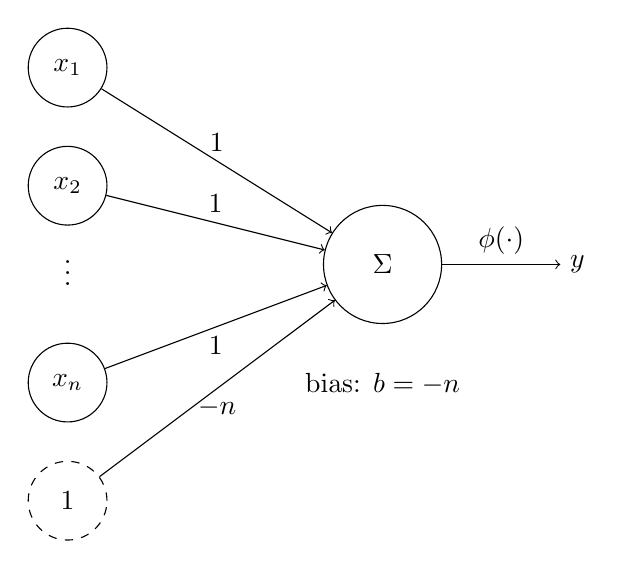
\begin{tikzpicture}[scale=1, transform shape]
			% Input nodes
			\node[circle, draw, minimum size=1cm] (x1) at (0, 3) {$x_1$};
			\node[circle, draw, minimum size=1cm] (x2) at (0, 1.5) {$x_2$};
			\node at (0, 0.5) {$\vdots$};
			\node[circle, draw, minimum size=1cm] (xn) at (0, -1) {$x_n$};
			\node[circle, draw, minimum size=1cm, dashed] (b) at (0, -2.5) {$1$}; % Bias input
			
			% Neuron
			\node[circle, draw, minimum size=1.5cm] (neuron) at (4, 0.5) {$\Sigma$};
			
			% Output
			\node[right=1.5cm of neuron] (out) {$y$};
			
			% Connections
			\draw[->] (x1) -- (neuron) node[midway, above] {$1$};
			\draw[->] (x2) -- (neuron) node[midway, above] {$1$};
			\draw[->] (xn) -- (neuron) node[midway, below] {$1$};
			\draw[->] (b) -- (neuron) node[midway, below] {$-n$};
			\draw[->] (neuron) -- (out) node[midway, above] {$\phi(\cdot)$};
			
			\node[below=0.5cm of neuron] {bias: $b=-n$};
		\end{tikzpicture}
		\end{latin}
		\caption{شبکه عصبی تک لایه برای تابع \lr{AND}}
	\end{figure}
	
	\subsection*{ب) پیاده‌سازی تابع \lr{OR} با $n$ ورودی}
	تابع \lr{OR} زمانی خروجی ۱ می‌دهد که \textbf{حداقل یک} ورودی برابر با ۱ باشد. تنها زمانی خروجی ۰ است که تمام ورودی‌ها ۰ باشند.
	
	مشابه حالت قبل، وزن‌ها را ۱ در نظر می‌گیریم ($w_i = 1$).
	شرایط مرزی:
	\begin{enumerate}
		\item اگر تمام ورودی‌ها ۰ باشند (مجموع ۰): خروجی باید ۰ باشد.
		$$ 0 + b < 0 \implies b < 0 $$
		\item اگر حداقل یک ورودی ۱ باشد (مجموع $\ge 1$): خروجی باید ۱ باشد.
		$$ 1 + b \ge 0 \implies b \ge -1 $$
	\end{enumerate}
	
	با انتخاب $b = -1$ شرط دوم ($1 - 1 = 0 \ge 0$) برقرار می‌شود و شرط اول ($0 - 1 = -1 < 0$) نیز صحیح است. (همچنین می‌توان $b=-0.5$ را نیز انتخاب کرد).
	بنابراین پارامترها:
	$$ w_i = 1, \quad b = -1 $$
	
	\begin{figure}[H]
		\centering
		\begin{latin}		
		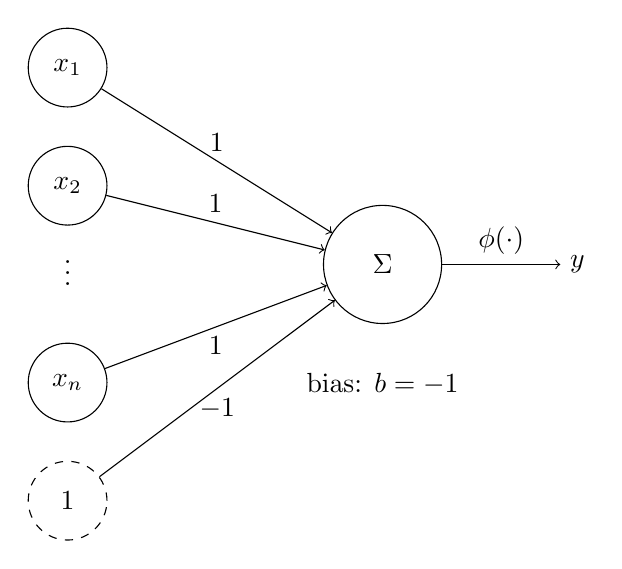
\begin{tikzpicture}[scale=1, transform shape]
			% Input nodes
			\node[circle, draw, minimum size=1cm] (x1) at (0, 3) {$x_1$};
			\node[circle, draw, minimum size=1cm] (x2) at (0, 1.5) {$x_2$};
			\node at (0, 0.5) {$\vdots$};
			\node[circle, draw, minimum size=1cm] (xn) at (0, -1) {$x_n$};
			\node[circle, draw, minimum size=1cm, dashed] (b) at (0, -2.5) {$1$}; % Bias input
			
			% Neuron
			\node[circle, draw, minimum size=1.5cm] (neuron) at (4, 0.5) {$\Sigma$};
			
			% Output
			\node[right=1.5cm of neuron] (out) {$y$};
			
			% Connections
			\draw[->] (x1) -- (neuron) node[midway, above] {$1$};
			\draw[->] (x2) -- (neuron) node[midway, above] {$1$};
			\draw[->] (xn) -- (neuron) node[midway, below] {$1$};
			\draw[->] (b) -- (neuron) node[midway, below] {$-1$};
			\draw[->] (neuron) -- (out) node[midway, above] {$\phi(\cdot)$};
			
			\node[below=0.5cm of neuron] {bias: $b=-1$};
		\end{tikzpicture}
		\end{latin}
		\caption{شبکه عصبی تک لایه برای تابع \lr{OR}}
	\end{figure}
	
	\subsection*{ج) عدم امکان پیاده‌سازی \lr{XOR} با کمتر از دو لایه}
	تابع \lr{XOR} (یا "یا انحصاری") برای دو ورودی باینری به صورت زیر تعریف می‌شود:
	\begin{itemize}
		\item $(0, 0) \to 0$
		\item $(1, 1) \to 0$
		\item $(0, 1) \to 1$
		\item $(1, 0) \to 1$
	\end{itemize}
	
	فرض کنیم یک پرسپترون تک لایه با وزن‌های $w_1, w_2$ و بایاس $b$ وجود داشته باشد که بتواند این تابع را پیاده‌سازی کند. روابط زیر باید برقرار باشند:
	\begin{enumerate}
		\item برای $(0,0)$: $0.w_1 + 0.w_2 + b < 0 \implies b < 0$
		\item برای $(1,1)$: $1.w_1 + 1.w_2 + b < 0 \implies w_1 + w_2 + b < 0$
		\item برای $(0,1)$: $0.w_1 + 1.w_2 + b \ge 0 \implies w_2 + b \ge 0$
		\item برای $(1,0)$: $1.w_1 + 0.w_2 + b \ge 0 \implies w_1 + b \ge 0$
	\end{enumerate}
	
	اگر نامساوی‌های (3) و (4) را با هم جمع کنیم:
	$$ (w_2 + b) + (w_1 + b) \ge 0 \implies w_1 + w_2 + 2b \ge 0 $$
	
	از طرفی طبق نامساوی (1)، $b$ عددی منفی است. بنابراین اگر $b$ را از عبارت فوق کم کنیم، سمت چپ بزرگتر می‌شود:
	$$ w_1 + w_2 + b > w_1 + w_2 + 2b \ge 0 $$
	$$ \implies w_1 + w_2 + b > 0 $$
	
	این نتیجه با نامساوی (2) که می‌گوید $w_1 + w_2 + b < 0$ در تناقض است.
	بنابراین هیچ خط راستی وجود ندارد که بتواند کلاس‌های خروجی ۰ و ۱ را در مسئله \lr{XOR} از هم جدا کند (مسئله به صورت خطی تفکیک‌پذیر نیست). برای حل این مشکل حداقل به یک لایه مخفی (یعنی شبکه دو لایه) نیاز است.
	
	\subsection*{د) معایب تابع پله‌ای و مزیت \lr{Sigmoid}}
	\textbf{چرا استفاده نمی‌شود؟}
	مشکل اصلی تابع فعال‌سازی پله‌ای (Step Function) در فرآیند آموزش شبکه است. الگوریتم‌های آموزش مدرن مانند «پس‌انتشار خطا» (\lr{Backpropagation}) بر پایه محاسبه گرادیان (مشتق) تابع هزینه نسبت به وزن‌ها عمل می‌کنند.
	مشتق تابع پله‌ای در تمام نقاط (به جز صفر) برابر با صفر است و در نقطه صفر نیز تعریف نشده است (ضربه).
	$$ \frac{d\phi}{dx} = 0 \quad (\text{for } x \ne 0) $$
	وقتی مشتق صفر باشد، گرادیان صفر می‌شود و وزن‌ها به‌روزرسانی نمی‌شوند، در نتیجه شبکه چیزی یاد نمی‌گیرد.
	
	\textbf{مزیت تابع \lr{Sigmoid}:}
	\begin{enumerate}
		\item \textbf{مشتق‌پذیری:} تابع سیگموئید ($ \sigma(x) = \frac{1}{1+e^{-x}} $) در تمام دامنه خود مشتق‌پذیر و پیوسته است.
		\item \textbf{گرادیان غیرصفر:} مشتق آن همواره غیرصفر است (هرچند ممکن است کوچک شود)، که اجازه می‌دهد سیگنال خطا به لایه‌های عقب‌تر منتشر شود.
		\item \textbf{غیرخطی بودن نرم:} گذار نرم بین ۰ و ۱ ایجاد می‌کند که برای تقریب توابع پیچیده و احتمالات مناسب‌تر است.
	\end{enumerate}
	
\end{document}